\documentclass[11pt,a4paper]{ivoa}
\input tthdefs
\lstset{flexiblecolumns=true}
\usepackage{todonotes}
\usepackage{array}
\usepackage{float}
\marginparwidth=4cm

\title{VO DCAT interface}

% see ivoatexDoc for what group names to use here
\ivoagroup{Registry}


\author{G.Landais}
\author{B.Cecconi}

\editor{G.Landais}

%\previousversion{This is the first public release}


\begin{document}
\begin{abstract}
	The document explores the W3C  DCAT (Data Catalogue) vocabulary in order to improve the harvesting of IVOA registry records within the Open Data landscape. It proposes a mapping of ivoa registry schemas with DCAT and focuses on the XML-RDF serialization which can be integrated into OAI-PMH output.
\end{abstract}


\section*{Acknowledgments}

\section*{Conformance-related definitions}


\section{Motivation}
\subsection{State of the art}
The registry of the Virtual Observatory \cite{std:registry} is distinctive in that it lists resources — whether datasets or services — that are closely linked with relationships. It has been created to be machine-readable allowing libraries or softwares to discover and query resources.

Data-centers provide resources which are collected by full registry \ref{rec:registry-interface}. The harvesting mechanism uses OAI-PMH with metadata described by standardized schemas like  VOResources \cite{std:2018ivoa.spec.0625P} (prefixe vr) and VODataServices \cite{std:vodataservice} (prefix vs) which draw the most important blocs. Each of these standards have XSD documents that allow the OAI-PMH XML serialization.
 
Full registries provide the whole resources through interfaces: the RegTAP interface which is generally used in the VO ecosystem (eg: pyvo registry module) and OAI-PMH interface allowing incremental harvesting.

For instance, EUDAT B2find is an interdisciplinary service  that harvests the vo registry with OAI-PMH. It makes the mapping between VO schemas and its own schema. The VO resources distributed in EUDAT don't include the whole VO schema; metadata like the coverage or services-datasets relations are removed or underused.

\subsection{DCAT}
The DCAT vocabulary \cite{dcat} \footnote{https://www.w3.org/TR/vocab-dcat-3/} is a W3C standard. It is a web semantic which, like the Registry schemas, allows to describe both DataSets and Services.

DCAT vocabulary reuse existing vocabulary like the RDF schema (prefix rdfs), the dublincore (prefix dct) or the friend-of-a-friend schema (prefix foaf), the whole completed with a DCAT vocabulary (prefix dcat).\\


DCAT provides a structured vocabulary and a primary class called \textit{dcat:Resource}. The \textit{dcat:Resource} class gathers basics metadata covering the \textit{vr:Curation} item. It is not intended to be used directly, it is preferred to use derived classes: 
\begin{itemize}
	\item \textbf{dcat:DataSet} is a set of data grouped in the same entity.
	\item \textbf{dcat:DataService} describes a WEB service (or a collection of services) giving access to one or more Datasets. It includes a endpoint URL and APIs description.
	\item \textbf{dcat:Catalogue} is a dcat:DataSet extension including additional metadata. It is a collection of Datasets or services, with common metadata, curated or provides by the same agent or organization.
	\item \textbf{dcat:DatasetSeries} is a dcat:DataSet extension including additional metadata. It is a collection of Datasets  that are published separately.
\end{itemize}
 
 \begin{figure}[htbp]
 	\label{diag-dcat}
 	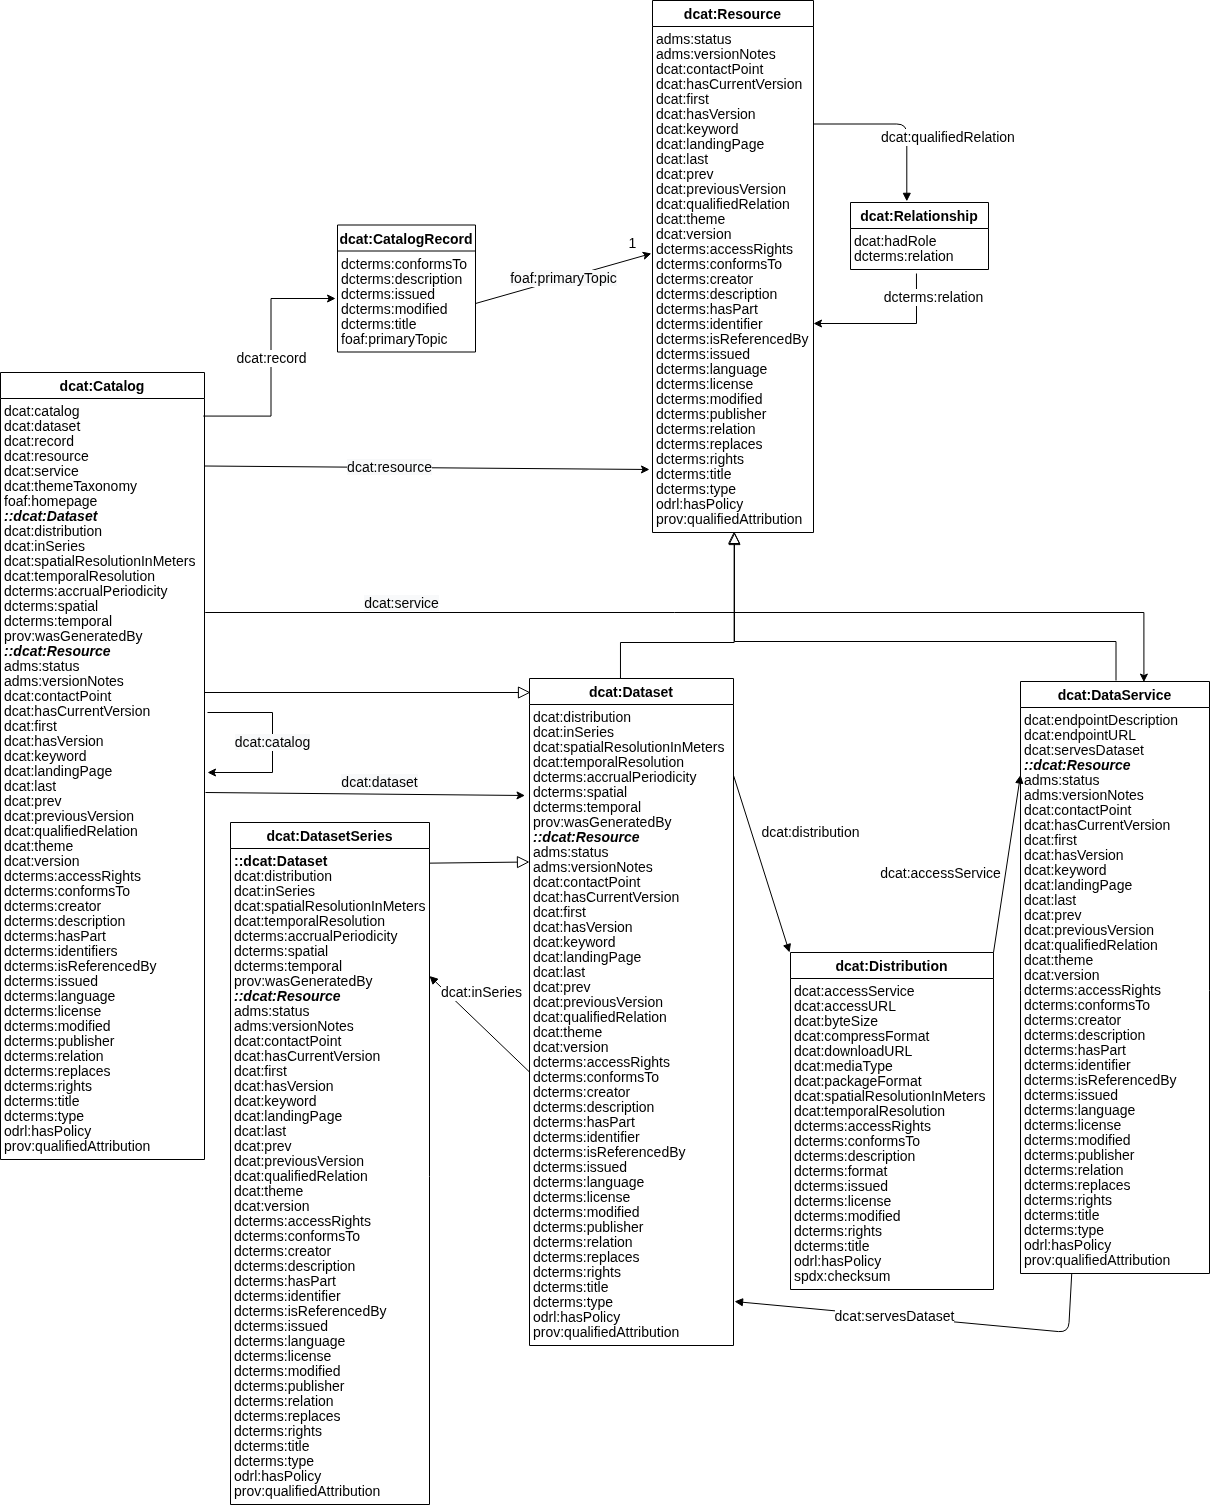
\includegraphics[width=1.2\textwidth]{dcat-schema-v3.png}
 	\caption{Overview of DCAT schema, figure coming from W3C document}%, \url{https://www.w3.org/TR/vocab-dcat-3/}}}
 \end{figure}
 
The relation connecting the classes together are represented in the diagram \ref{diag-dcat}. 

\subsubsection{DCAT Services and distributions}
In DCAT, the distribution is an access to a form of a DataSet. It can be a Download URL (an endoint URL) or an API served by a Service.

There are different serialization to map the access and the Dataset.\\

\begin{enumerate}
	\item \label{Collection-service} \textbf{Service belonging to a Collection}:
     declare a service (\textit{dcat:DataService}) which belongs to a dcat:Catalogue.
	\item \label{dataset-distribution} \textbf{Dataset with Distribution}:
	use distributions (\textit{dcat:Distribution class}) for each data (for example Zenodo uses a distribution for each files of the dataset). Distribution are also used  to declare the different accesses of a same data available in different form (fomat CSV, XML, etc). 
	This method is used basically for download URLs.
	\item  \label{dataset-combine} \textbf{Dataset distributed by a Service}: use distribution by specifying \textit{dcat:DataService}. This method is basically used to data requiring a web page or an API.   
\end{enumerate}
 
\subsubsection{DCAT Serialization}

The DCAT vocabulary which combines Collection, DataSet, accessURL and Service requires the provider to make some choice in the serialization.

For instance, a Zenodo\footnote{\url{https://zenodo.org/}} deposit possibly contains several resources with  metadata applying for the whole deposit. Zenodo chose \textit{dcat:DataSet} for the deposit and use distributions to access by URL each resource.

In this document, we propose to use \textit{dcat:Catalogue} and \textit{dcat:DataService} to describe API.


\subsection{DCAT usage}
DCAT is a reference to map datasets in Open Data. It is widely used to both expose and harvest metadata:

 \begin{itemize}
\item google datasetsearch consumes JSON-LD metadata included in landingpage. It accepts the schemas schema.org or DCAT.
\item Zenodo provides a DCAT export for its deposits. It includes the DCAT serialization in the XML OAI-PMH (metadataPrefix=DCAT).
\item The EOSC EU node \footnote{\url{https://open-science-cloud.ec.europa.eu/}} chose DCAT as prefered schema for harveting. 
\end{itemize}



\subsection{DCAT extensions}
DCAT schema has been adopted by many organizations and by many purposes. 
It is used in its original form or by adding extensions.

\begin{itemize}
\item In Europe, DCAT-AP (DCAT Application Profile) \footnote{https://semiceu.github.io/DCAT-AP/releases/3.0.0/} extends the schema with legislation metadata and is a basis for customized DCAT schemas. It includes new attributes such as availability and set some attributes to be mandatory. For instance:
\begin{itemize}
	\item geoDCAT-AP extends DCAT for geospatial data
	\item StatDCAT-AP extends DCAT for statistics data
\end{itemize} 

\item US-DCAT extends the access URL and conformance attribute. It adds also a list of new concept such as Quality Measurement and legal attributes.
\end{itemize}

\section{VODcat mapping}

VODcat is a DCAT serialization which includes additional vocabulary and classes coming from the Registry.

\subsection{Limitation and addition}
DCAT schema includes a part of the registry metadata. For instance it includes global metadata \textit{vr:Curation} and \textit{vr:Content}, an important part of the \textit{vr:Capability} but it doesn't include other metadata like \textit{vs:Coverage}, \textit{vs:Table} definition. \\

The VODcat serialization includes VODataService XSD URL in the $<$ri:metadata$>$ of the OAI document(see appendix \ref{namespace}).

 \begin{figure}[htbp]
	\label{diag-vodcat}
	\includegraphics[width=1.2\textwidth]{vodcat-schema.png}
	\caption{VODcat schema}
\end{figure}



\subsection{Pre-requisite and choices}

\textbf{Note}: in order to provide an interfaces usable in an interdisciplinary perspective, the mapping has been influenced by Zenodo DCAT implementation.\\

List of VODcat choices:

\begin{itemize}
	\item Use and declare RDF-XML DCAT serialization in $<$ri:metadata$>$ of the OAI-PMH records.
	\item Adopt Zenodo extension to include additional DataCite attributes (prefix citedcat) \footnote{https://w3id.org/citedcat-ap}
	\item Choose the following primary classes 
	    \begin{itemize}
		\item \textit{dcat:DataService} for \textit{vs:DataService}
		\item \textit{dcat:Catalogue} for \textit{vs:DataResource}
		\item \textit{dcat:Catalogue} for \textit{vs:CatalogueService}
		\item \textit{dcat:Catalogue} for \textit{vs:CatalogueResource}
		\end{itemize}
	\item Use \textit{dcat:Dataset} for each \textit{vs:Table}. Each Dataset is attached to the registry record (\textit{dcat:Catalog}) with  \textit{dcat:dataset} property.
	
	\textbf{Note}: this mapping differs to Zenodo which choose for its deposit \textit{dcat:DataSet} and \textit{dcat:Distribution} for all of these data. But Zenodo does not provide API and tableset defintions. 

	\item Use both \textit{dcat:Distribution} and its property \textit{dcat:accessService} to \textit{vr:Capabilities} (see \ref{dataset-combine} or \ref{dataset-distribution})

	
	\item When possible, attach \textit{dcat:Distribution} to the \textit{dcat:Dataset} Table.
	
	\item Focus on  \textit{vr:Interfaces} having standardId (other are options)
	\item Extends DCAT with VODataService to add the \textit{vs:TableSet} and \textit{vs:Coverage}.
	
    \item (OBSOLETE) Use \textit{rdf:Description} in XML in order to be compatible with RDF semantic (allow to convert the $<$ri:metadata$>$ XML into JSON-LD or Turtle)

\end{itemize}

\subsection{Mapping}

This mapping has been implemented by an XSLT document that transforms VO registry record in DCAT.   
The mapping supports $<$ri:metadata$>$ content to any RDF format (JSON-LD, Turtle).\\


\textbf{Warning}: to be fully RDF compliant, all schema used in the serialization should be in RDF. The VO XSD schemas (eg: VODataService) should be mapped into RDF document (in Turtle for instance).
At the time of the writing of this document, the work has been initiated by the Paris Observatory \footnote{IVOA presentation of Liza Fretel at https://wiki.ivoa.net/twiki/bin/view/IVOA/InterOpJun2026Semantics}

\subsubsection{Curation}

\textcolor{red}{is it needed to explain what is Range?}\\
\begin{tabular}{|l|l|l|l|} \hline
	\textbf{Registry element} & \textbf{Parent Registry class} & \textbf{DCAT}  \\ \hline
	vr:publisher &  vr:ResourceName & dct:publisher (*)  \\ \hline 
	vr:Creator & vr:Creator & dct:creator (*) \\ \hline 
	vr:Contributor & vr:ResourceName & dct:contributor (*) \\ \hline 
	vr:date[@role='Created'] & vr:Date& dct:created \\ \hline
	vr:date[@role='Updated'] & vr:Date& dct:modified \\ \hline
    oai:identifier & & adms:identifier (*)\\ \hline
    vr:altIdentifier & vr:ResourceName & adms:identifier (*) \\ \hline
    vr:shortName & vr:ShortName & \textcolor{red}{dct:identifier ?}\\ \hline
    vr:contact & vr:Contact & dcat:contactPoint(*)\\ \hline
    
\end{tabular}\\

\paragraph{About dct:publisher} (\textit{foaf:Agent} range): Use \textit{foaf:nick} when \textit{@vr:altIdentifier} is specified.

\paragraph{About dct:curator and dct:creator} (\textit{foaf:Agent} range):  specifies the type "Organisation" or "Person" in an encapsulated \textit{rdf:Description} (same method is used by Zenodo).\\
By default, use the type \textit{foaf:Person} when \textit{@vr:altIdentifier} is not prefixed by ivoid or RoR.
When exists, the ORCID (\textit{@vr:altIdentifier}) is added in \textit{@rdf:about} attribute.\\

Example:
\begin{lstlisting}
<dct:creator>
    <rdf:Description rdf:about="orcid:0000-0003-0081-1797">
        <rdf:type rdf:resource="https://xmlns.com/foaf/0.1/Person"/>
        <foaf:name>Bryson S.</foaf:name>
    </rdf:Description>
</dct:creator>
\end{lstlisting}

\paragraph{About adms:identifier}: use \textit{adms:identifier} only for alternate identifier that uses the ivoid or DOI scheme (other are skipped). Use property \textit{adms:schemaAgency} to secify the scheme (as Zenodo). 

\paragraph{About dcat:contactPoint}:
use \textit{vcard:Organization} with property \textit{vcard:fn} for name, \textit{vcard:address} (equivalent to \textit{vcard:hasAddress} but accepting Litteral) for address and \textit{vcard:email} for email.


\subsubsection{Content}

\begin{tabular}{|l|l|l|} \hline
	\textbf{Registry element} & \textbf{Parent Registry class} & \textbf{DCAT}  \\ \hline
	vr:subject & xs:token & dct:description \\ \hline
	vr:source & vr:Source & citedcat:isSupplementTo (*)\\ \hline
	vr:referenceURL & & dcat:landingpage \\ \hline
	vr:type & xs:token & dct:type (*)\\ \hline
    vr:contentLevel & xs:token & adms:status (*)\\ \hline
	vr:rights & vr:Rights & dct:rights\\ \hline
\end{tabular}    

\paragraph{About citedcat:isSupplementTo}:
Encapsulate the relation in an \textit{rdf:Description}. Specifies the identifier in \textit{@rf:about} attribute with DOI or bibcode (prefix the bibcode with ADS URL). We assume that the identifier is a bibcode for any alternate identifier having no prefix.
The relation is completed with \textit{dct:identifier} and  \textit{rdf:type} \url{https://www.ivoa.net/rdf/voresource/content_type/content_type.html#Bibliography}

\paragraph{About dct:type}: use the IVOA vocabulary with URL: \url{http://www.ivoa.net/rdf/voresource/content_type#{type}}

\paragraph{About adms:status}: use the IVOA vocabulary with URL: \url{http://www.ivoa.net/rdf/voresource/content_level#{type}}



\subsubsection{Declare interface}
For each \textit{vr:Interface}, we use Distribution (see method \ref{dataset-combine}).

\begin{itemize}
	\item  use distribution on \textit{dcat:Catalog} level when the service (ie: \textit{vs:interface}) serves one or more tables without giving exactly which table(s).\\
	\begin{figure}[htbp]
		
\includegraphics[width=\textwidth]{dcat-catalog-distrib.png}
		\caption{Capability/Interface attached to \textit{dcat:Catalog}}
	\end{figure}
	This method is adapted to service such as TAP which serve the tables listed in the registry record or when the relation Interface-Table is not defined.
	
	\item  use distribution on \textit{dcat:Dataset} level when the service (ie: \textit{vs:interface}) serves only the current table.\\
	\begin{figure}[htbp]
		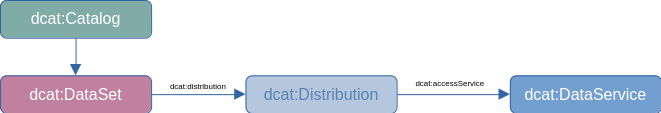
\includegraphics[width=\textwidth]{dcat-dataset-distrib.png}
		\caption{Capability/Interface attached to \textit{dcat:Dataset}}
	\end{figure}
	This option is better to link services and tables. However, the method is today difficult to implement because there is no clean methods today in the registry to link interfaces and tables.\\
	
	
	A first step has been proposed in VODataService 1.3 that allows \textit{vs:Interface} to declare HTTP parameters and values (see VODataService with \textit{vs:stats} in Interface). Then, standards protocols (eg: SCS2) including parameter "TABLE" allows to link the \textit{vs:Interface} with \textit{vs:Tables} using table name (case (2))
	
	
	\begin{lstlisting}
	<interface xsi:type="vs:ParamHTTP" role="std">
	  <accessURL use="base">https://anyURL</accessURL>
	  <inputParam name='TABLE'>
	    <stats>
	      <option>J/AJ/167/21/table1</option>
	    </stats>
	  </inputParam>
	</interface>
	\end{lstlisting}
	
	\item use distribution on \textit{dcat:Catalog} level when the Service serves multiple tables and when the relations Interfaces-Tables is established.\\
	This possibility is an alternative of the previous note. \\
	\begin{figure}[htbp]
		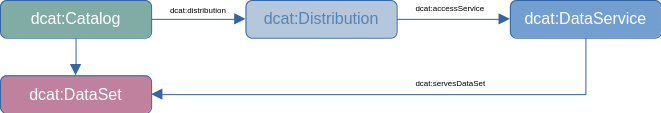
\includegraphics[width=\textwidth]{dcat-catalog-dataset-distrib.png}
		\caption{Capability/Interface attached to \textit{dcat:Catalog} that serve a list of \textit{dcat:DataSet}}
	\end{figure}
	
\end{itemize}



\paragraph{Note}: use similar serialization for mirrors (\textit{vr:mirrorURL}).

\subsubsection{RelationShips}

\textcolor{red}{TODO continue with other relation? or skip ?}

\textbf{Warning} Add only relations having an ivo-id.\\


\begin{tabular}{|l|l|l|} \hline
    \textbf{relationShipType} & \textbf{Parent Registry class} & \textbf{DCAT}  \\ \hline
    isServedBy (*) & vr:RelationShip&  dcat:distribution\\ \hline
    isSupplementTo & vr:RelationShip& citedcat:isSupplementTo \\ \hline
    Cites   & vr:RelationShip& bibo:Cites \\ \hline
    \textit{any others ...} & vr:RelationShip & dct:relation \\ \hline
\end{tabular}

 
\paragraph{isServedBy relation}:\\
%\textbf{Warning} declare here the ivo service (only). Do not specify by this way the vr: capability.\\
\textbf{Warning} declare only service having ivoi-id in registry element.\\

\begin{figure}[htbp]
	
\includegraphics[width=\textwidth]{dcat-catalog-distrib-remote.png}
%\caption{Relation vr:isServedby using dcat:Distribution. The service is described in external resource}
\end{figure}

The mapping uses \textit{dcat:Distribution} as described in method \ref{dataset-combine} with specifying the ivoid of the service and an empty \textit{dcat:DataService}.

\paragraph{Other relations}: \\
Relation \textit{dcat:relation} are encapsulated into \textit{rdf:Description} with \textit{@rdf:about} attribute for DOI or ivoid identifier. 
The relation is completed with optional \textit{rdf:type} (\url{http://www.w3.org/ns/dcat#DataSet}) and \textit{dct:identifier} when it is known. 

\subsubsection{Coverage}
The coverage uses the VODataService extension (\textit{vs:Coverage}).
The content is a copy of the existing registry coverage. % encapsulated into an \textit{rdf:Description} (to ensure RDF compatibility).

Example:
\begin{lstlisting}
<vs:coverage>
    <vs:Coverage>
        <vs:spatial>...</vs:spatial>
        <vs:footptint>...</vs:footprint>
        <vs:waveband>...<vs:waveband>
    </vs:Coverage>
</vs:coverage>
\end{lstlisting}

\subsubsection{Declare tableset}
Table declaration is only possible in the VODcat extension (and not in DCAT) with declaring VODataService (prefix vs in the XML document).\\

Example:

\begin{lstlisting}
<dcat:catalog>
    <dcat:DataSet>
        <dct:identifier>I/350/gaiaedr3</dct:identifier>
        <vs:table>
	        <vs:Table>
	            <vs:name>I/350/gaiaedr3</ivods:name>
	            ...
	            <vs:column>
	                <vs:Column>
	                    <vs:name>Plx</ivods:name>
	                    <vs:ucd>pos.parallax.trig</ivods:ucd>
	                    ....
	                </vs:Columnn>
	            </vs:column>    
	            ....
            </vs:Table>
        </vs:table>
    </dcat:DataSet>
    ...
</dcat:catalog>
\end{lstlisting}


\section{Declaring DCAT as prefix in VO Registries}
OAI-PMH protocole allows different metadata prefix. The DublinCore (prefix oai\_dc) and the IVOA prefix (ivo\_vor) are mandatory in the VO registry.\\

We propose a new optional prefix dcat that has to be used if DCAT is available in the output of the OAI-PMH provided by the registry. This added prefix can be added to any registry. However, because the DCAT output doesn't cover the full metadata existing with the ivo\_vor prefix, it should not be used by full-registry harvesting.\\
 
 
 The new prefix must be listed in the OAI-PMH query 'verb=ListMetadataFormats'.
 Example: \url{http://rofr.ivoa.net/oai?verb=ListMetadataFormats}
 
Declaration of the DCAT Prefix element in OAI-PMH. \begin{lstlisting}
<metadataFormat>
  <metadataPrefix>dcat</metadataPrefix>
  <schema>http://schema.datacite.org/meta/kernel-4/metadata.xsd</schema>
  <metadataNamespace>https://www.w3.org/ns/dcat</metadataNamespace>
</metadataFormat>
\end{lstlisting}
 
\appendix
\section{Appendix, Changes from Previous Versions}
RAS

\subsection{Appendix: Namespaces declaration}

\label{namespace}
\begin{tabular}{|l|l|} \hline
\textbf{name} & \textbf{URI} \\  \hline
rdf &http://www.w3.org/1999/02/22-rdf-syntax-ns\\ \hline
adms &http://www.w3.org/ns/adms\#  \\ \hline
bibo &http://purl.org/ontology/bibo/ \\ \hline 
citedcat &https://w3id.org/citedcat-ap \\ \hline 
dct &http://purl.org/dc/terms/ \\ \hline 
dctype &http://purl.org/dc/dcmitype/ \\ \hline 
dcat &http://www.w3.org/ns/dcat\# \\ \hline 
foaf &http://xmlns.com/foaf/0.1/ \\ \hline
gsp &http://www.opengis.net/ont/geosparql\# \\ \hline
locn &http://www.w3.org/ns/locn\# \\ \hline
org &http://www.w3.org/ns/org\# \\ \hline
owl &http://www.w3.org/2002/07/owl\# \\ \hline
prov &http://www.w3.org/ns/prov\# \\ \hline
rdfs &http://www.w3.org/2000/01/rdf-schema\# \\ \hline
skos &http://www.w3.org/2004/02/skos/core\# \\ \hline
vcard &http://www.w3.org/2006/vcard/ns\# \\ \hline
wdrs &http://www.w3.org/2007/05/powder-s\# \\ \hline 
vs &\color{red}{http://www.ivoa.net/xml/VODataService/v1.1\#} (*)\\ \hline
\end{tabular}

(*) VO addition for coverage and tableset.


\subsection{Appendix: example of VODcat distribution}:\\

Example: Service attached to the whole \textit{dcat:Catalog}


\begin{lstlisting}
<dcat:Catalog>
  ..
  <dcat:distribution>
	<dcat:Distribution>
	  <dct:description>
		Data access using the Simple Cone Search
	  </dct:description>
	  <dcat:conformTo>ivo://ivoa.net/std/ConeSearch</dcat:conformTo>
	  <dct:formats>text/xml+votable</dct:formats>
	  <dcat:accessService>
		<dcat:DataService rdf:about="ivoid_of_the_service">
		  <dcat:endpointURL>https://anyurl?</dcat:endpointURL>
		  <dcat:endpointURLDescription>
			http://ivo.net/openAPI/...
		  </dcat:endpointURLDescription>
		</dcat:DataService>
	  </dcat:accessService>
	</dcat:Distribution>
  </dcat:distribution>
	...
</dcat:Catalog>
\end{lstlisting}


\bibliography{ivoatex/ivoabib,ivoatex/docrepo,local,VODcat}

\end{document}
